\documentclass[oneside]{book}

\usepackage[english]{babel}
\usepackage[T1]{fontenc} 
\usepackage[utf8]{inputenc}
\usepackage{amsmath}
\usepackage{amssymb}
\usepackage{amsfonts}
\usepackage{graphicx}
\usepackage[ruled]{algorithm2e}
\usepackage{empheq}
\usepackage{float}
\usepackage{listings}
\usepackage{color}
\usepackage{fullpage}

\setcounter{tocdepth}{4}
\setcounter{secnumdepth}{5}

\definecolor{dkgreen}{rgb}{0,0.6,0}
\definecolor{gray}{rgb}{0.5,0.5,0.5}
\definecolor{mauve}{rgb}{0.58,0,0.82}
\definecolor{blck}{rgb}{0,0,0}

\lstset{frame=tb,
  language=Java,
  keepspaces=true,
  aboveskip=3mm,
  belowskip=3mm,
  showstringspaces=false,
  columns=flexible,
  basicstyle={\small\ttfamily},
  numbers=none,
  numberstyle=\tiny\color{gray},
  keywordstyle=\color{blue},
  commentstyle=\color{dkgreen},
  stringstyle=\color{mauve},
  breaklines=true,
  breakatwhitespace=true
  tabsize=3
}

\title{Algorithmic Programming in Java}
\author{Rodion Efremov} 
\date{}

\begin{document}
\maketitle
\tableofcontents

\chapter*{Preface}
This book is aiming to provide insight into practical implementation of algorithms and data structures in a way that is as accessible to readers of all proficiency levels. Only very basic knowledge of Java programming language and other tools is assumed; wherever relevant, the new language features are explained succinctly without further ado. The book is organized in a ``bottom-up'' fashion so that the book is better read linearly, but not necessarily continuously whenever some topics do not interest. There is no exercises. Instead, the book presents the code listings for a Java library of algorithms and data structures, so the book might be used as a collection of ``algorithmic recipes''. 

The second objective is to provide a gentle introduction to formalism taking place in computer science independent of particular tool sets. By formalism we mean most often pseudo-code, big O notation, set notation, sequences and functions. We, however, will not do any fancy mathematics with Greek letters such as proving theorems, etc. Whether to learn formalism or not mainly depends on your academic aims: in case you are planning to enroll in a department of computer science, this book just might be everything you need to get prepared for your studies.

\makeatletter\@openrightfalse
\part{Introduction}
This part will introduce the reader to common ground for successive parts of the book. The topics covered are coding conventions for the library we will implement, using \textbf{Maven} to manage your version of the library, and using \textbf{git} to store your version of the library.

\chapter{Coding conventions and tools}
\@openrighttrue\makeatother
\section{Naming types, methods and variables}
The Java community encourages using ``CameCase'' to name your identifiers. For instance, \texttt{elementAmount}, \texttt{nodePriority} are identifiers for local variables or class fields adhering to CamelCase style. Following the intuition, \texttt{getSize} or \texttt{decreasePriority} are (in some sense) ``good'' names for class methods. The naming convention for user-defined types makes a small exception to the above rule: the first letter is capitalized: \texttt{PathFinder}, \texttt{DirectedGraphNode}.

\section{Fluent API}
While developing a software library $L$, the top priority is keeping $L$'s API (application programming interface) as simple as possible. Simplicity does not come automatically with the presence of Javadoc\footnote{A documenting tool included in Java Development Kit.} for each class in $L$. Consider the following code snippet:
\begin{lstlisting}
Node source = ...;
Node target = ...;
Path<Node> p = new DijkstraFinder<Node>().search(source, target);
\end{lstlisting}
\newpage
\noindent This is intuitive and easy to remember. On the contrary, the following is not quite:
\begin{lstlisting}[caption={Too much arguments for a method call},label=lst:bidirastarfinder1]
Node source = ...;
Node target = ...;
PriorityQueue<Node> queue = ...;
HeuristicFunction<Node> h1 = ...;
HeuristicFunction<Node> h2 = ...;
Path<Node> p = new BidirectionalAStarFinder<Node>().search(source, 
							   target, 
							   queue, 
							   h1, 
							   h2);
\end{lstlisting}
There is a way to make an API more convenient, and it is usually called ``fluent'' API, where a call to a function is prepared argument by argument in the following manner:
\begin{lstlisting}
Path<Node> p = usingBidirectionalAStarFinder<Node>
              .from(source)
              .to(target)
              .withPriorityQueue(queue)
              .withForwardHeuristic(h1)
              .withBackwardsHeuristic(h2)
              .search();
\end{lstlisting}
The above listing is an improvement over Listing \ref{lst:bidirastarfinder1}.
Now that we know the name of the technique, let's see a working example:
\lstset{
  numbers=left
}
\begin{lstlisting}
public class Main {
    
    public static void main(String... args) {
        String result1 = begin().withSource("France")
                                .withTarget("Japan")
                                .withAlgorithm1();
        
        String result2 = begin().withSource("Germany")
                                .withTarget("Finland")
                                .withAlgorithm2();
        
        System.out.println(result1);
        System.out.println(result2);
    }
    
    static SourceNodeSelector begin() {
        return new SourceNodeSelector();
    }
}

abstract class Algorithm {
    protected TargetNodeSelector targetNodeSelector;
    
    abstract String execute();
    
    Algorithm(TargetNodeSelector targetNodeSelector) {
        this.targetNodeSelector = targetNodeSelector;
    }
}

class Algorithm1 extends Algorithm {
    
    Algorithm1(TargetNodeSelector targetNodeSelector) {
        super(targetNodeSelector);
    }
    
    String execute() {
        return "ALGORITHM1 from " + targetNodeSelector.getSource() + " to " +
               targetNodeSelector.getTarget();
    }
}

class Algorithm2 extends Algorithm {
    
    Algorithm2(TargetNodeSelector targetNodeSelector) {
        super(targetNodeSelector);
    }
    
    String execute() {
        return "ALGORITHM2 from " + targetNodeSelector.getSource() + " to " +
                targetNodeSelector.getTarget();
    }
}

class SourceNodeSelector {
    private String source;
    
    TargetNodeSelector withSource(String source) {
        this.source = source;
        return new TargetNodeSelector(this);
    }
    
    String getSource() {
        return source;
    }
}

class TargetNodeSelector {
    private SourceNodeSelector sourceNodeSelector;
    private String target;
    
    TargetNodeSelector(SourceNodeSelector sourceNodeSelector) {
        this.sourceNodeSelector = sourceNodeSelector;
    }
    
    AlgorithmSelector withTarget(String target) {
        this.target = target;
        return new AlgorithmSelector(this);
    }
    
    SourceNodeSelector getSourceNodeSelector() {
        return sourceNodeSelector;
    }
    
    String getSource() {
        return sourceNodeSelector.getSource();
    }
    
    String getTarget() {
        return target;
    }
}

class AlgorithmSelector {
    private TargetNodeSelector targetNodeSelector;
    
    AlgorithmSelector(TargetNodeSelector targetNodeSelector) {
        this.targetNodeSelector = targetNodeSelector;
    } 
    
    public String withAlgorithm1() {
        return new Algorithm1(targetNodeSelector).execute();
    }
    
    public String withAlgorithm2() {
        return new Algorithm2(targetNodeSelector).execute();
    }
}
\end{lstlisting}
You can see a fluent API in action at lines 4 and 8. First of all, this is more explicit about the meaning of each argument passed to a method. Second point is the fact that the sequence of arguments being ``built'' is fixed, you cannot write \texttt{withTarget(...)} before \texttt{withSource(...)}. Also, you will get a compilation error whenever you forget to specify an argument of a fluent API call:
\newpage
\lstset{
numbers=none
}
\begin{lstlisting}[caption={Bad fluent API call},label=lst:badfluentapi]
begin().withSource("France")
       .withAlgorithm1();  // Compile-time error: withSource returns 
                           // TargetNodeSelector which has no 
                           // withAlgorithm1.
\end{lstlisting}
The last but not least, modern IDE's (integrated development environments) support code-completion, which makes it easier to write syntactically correct code. For instance, in Listing \ref{lst:badfluentapi}, a good IDE, after writing \\ \texttt{begin().withSource(...)}, will give a list of suggestions containing \texttt{withTarget} - method. That way, you don't need to remember each and every function, the IDE will guide you through making calls to a fluent API methods.

\section{Bare necessities}
\subsection{Using Maven for managing the projects}
Developing a library regardless of a language, usually results in dozens of files, which makes it inconvenient to work at the lowest level (invoking \textbf{javac} and \textbf{java} every time she or he recompiles a project). Maven is a build tool remedying the issue. First, we might want to create Maven-driven Java project:
\begin{verbatim}
mvn archetype:create -DgroupId=com.example -DartifactId=my-proj
\end{verbatim}
The above spell will take the current working directory and create in it a following file system tree:
\begin{center}
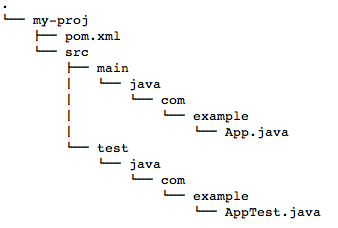
\includegraphics[width=240px,keepaspectratio]{mvntree}
\end{center}
If you look at it, you may guess that the file \textbf{pom.xml} configures the project we just created:
\lstset{
language=XML,
keywordstyle=\color{blck},
}
\begin{lstlisting}
<project xmlns="http://maven.apache.org/POM/4.0.0"
         xmlns:xsi="http://www.w3.org/2001/XMLSchema-instance"
         xsi:schemaLocation="http://maven.apache.org/POM/4.0.0
         http://maven.apache.org/xsd/maven-4.0.0.xsd">
  <modelVersion>4.0.0</modelVersion>

  <groupId>com.example</groupId>
  <artifactId>my-proj</artifactId>
  <version>1.0-SNAPSHOT</version>
  <packaging>jar</packaging>

  <name>my-proj</name>
  <url>http://maven.apache.org</url>

  <properties>
    <project.build.sourceEncoding>UTF-8</project.build.sourceEncoding>
  </properties>

  <dependencies>
    <dependency>
      <groupId>junit</groupId>
      <artifactId>junit</artifactId>
      <version>3.8.1</version>
      <scope>test</scope>
    </dependency>
  </dependencies>
</project>
\end{lstlisting}
Now, if we type \textbf{mvn test} from the directory \textbf{my-proj}, Maven will compile all the sources in the project and run all available tests. If we add the XML snippet in the Listing \ref{lst:mvnexecjava} into the \textbf{pom.xml} right after the \textbf{</dependencies>} closing tag, we could run the project simply by typing \textbf{mvn exec:java} in the directory containing the project's \textbf{pom.xml}.
\begin{lstlisting}[caption={Configuring Maven exec plugin},label=lst:mvnexecjava]
<build>
  <plugins>
    <plugin>
     <groupId>org.codehaus.mojo</groupId>
     <artifactId>exec-maven-plugin</artifactId>
     <version>1.3</version>
     <executions>
       <execution>
         <goals>
           <goal>java</goal>
         </goals>
       </execution>
      </executions>
      <configuration>
        <mainClass>com.example.App</mainClass>
      </configuration>
    </plugin>
  </plugins>
</build>
\end{lstlisting}

\subsection{Working with git}
The last tool we will discuss is \textbf{git}, a distributed source code management software. This is by no means mandatory for following this book, so if you don't need a place on Internet where you can store your code, feel free to omit this section.

\subsubsection{Basic git workflow}
The easiest way to maintain a \textbf{repository}\footnote{A file system subtree comprising a software project.} is to register at \textbf{github.com} and create a repository from the site's web interface. Suppose your nickname was \textbf{Sheila}, and you created a repository \textbf{spacer}. So as to put some code into her repository, Sheila would write from her terminal:
\begin{verbatim}
git init
git add . # (dot) as everything beginning from current directory
git commit -m "Your commit message"
git remote add origin git@github.com:Sheila/spacer.git
git push -u origin master
\end{verbatim}
Next, whenever Sheila modifies files in local instance of \textbf{spacer}, the following routine would update the repository at \textbf{github.com}:
\begin{verbatim}
git status # show which files where created/modified/removed
git add . 
git status
git commit -m "New commit message"
git push
\end{verbatim}
The second invocation of \textbf{git status} will show which files were included in a commit; if not already colorful, you might make the output of \textbf{git status} funkier by running from the console:
\begin{verbatim}
git config --global color.ui auto
\end{verbatim}
\part{Basic algorithms and data structures}  

\chapter{Fundamental algorithms}
In this chapter we will implement some very basic algorithms and establish their ``complexities''.

\section{Initializing a project}
Most Java programs and libraries a structured in class files and packages. The class files define classes (user-defined types), and whenever a user-defined type is called $T$, the file implementing $T$ is called $T$\textbf{.java}. Most of Java files belong to a package, which is ``implemented'' as a simple folder. Along Java files, a package may contain other packages. This structure does not, however, contain cycles, i.e. the source code of a Java software item is a \textbf{tree} somewhere in the file system. 

Every package should be named by a lower-case string, and the topmost package hierarchy should resemble the domain name of a business having developed the software: \textbf{com.coderodde.apij.graph}, \textbf{com.coderodde.apij.ds}, etc. 

As above, the three topmost packages of the library we will develop during the course of this book, are \textbf{com}, \textbf{com.coderodde} and \textbf{com.coderodde.apij}. You may choose whatever you want (for instance, $P$). So whenever you see \textbf{com.coderodde.apij}, just substitute it with your $P$.
\section{Generating data and searching}
Now, let's create a package \textbf{com.coderodde.apij.util} and add the file \textbf{Utils.java} to it:
\lstset{
language=Java,
numberstyle=\tiny\color{gray},
keywordstyle=\color{blue},
commentstyle=\color{dkgreen},
numbers=left}
\begin{lstlisting}
package com.coderodde.apij.util;

import java.util.Random;

public class Utils {
    
    public static final Integer[] getRandomIntegerArray(final int size,
                                                        final int min,
                                                        final int max,
                                                        final Random r) {
        checkMinMax(min, max);
        final Integer[] arr = new Integer[size];
        
        for (int i = 0; i < size; ++i) {
            arr[i] = r.nextInt(max - min + 1) + min;
        }
        
        return arr;
    }
    
    private static final <T extends Comparable<? super T>> void 
    checkMinMax(T min, T max) {
        if (min.compareTo(max) > 0) {
            // Here we have "min > max".
            throw new IllegalArgumentException("'min' is larger than 'max'.");
        }
    }
}
\end{lstlisting}
Because all but the most obvious methods will be explained in text, I will omit their respective javadoc comments. Now, the method \textbf{checkMinMax} maintains the invariant of \textbf{min} being no more than \textbf{max}, and if it fails, an exception with a message reporting the root cause is thrown. Actually, we could have omitted the entire check, but in the case the invariant ``$\textbf{min} \leq \textbf{max}$'' would have been invalidated, the exception would have been thrown on line 15 in the above listing; this is fine, but might be less obvious than the message originating from \textbf{checkMinMax}. We will stick to such defensive style as to provide the error messages as soon as possible and not ``$N$ calls later''.

Now, the method \textbf{getRandomIntegerArray} will generate an array of \textbf{size} \textbf{Integer} wrappers with each integer belonging to range $R = [\textbf{min}, \textbf{max}]$ (every element in $R$ is equiprobable).

Suppose we come up with an integer $i$, and we want to find the least index in the integer array having value $i$. The following algorithm scans through the array and as soon as it gets to an integer being equal to $i$, returns the index of that integer. (In case no match was found, it is conventional to return a negative index, such as $-1$, to indicate that.)
\begin{lstlisting}[caption={Linear search algorithm}]
    public static final int INDEX_NOT_FOUND = -1;
    
    public static final <T> int findIndexOf(final T[] array, final T element) {
        if (array == null) {
            return INDEX_NOT_FOUND;
        }
        
        for (int i = 0; i < array.length; ++i) {
            if (array[i].equals(element)) {
                return i;
            }
        }
        
        return INDEX_NOT_FOUND;
    }
\end{lstlisting}
\textbf{Utils.java} would be a good place for our linear search. What about order statistics such as minimum or maximum value in an array? That easiness belongs to \textbf{Utils.java} as well:
\begin{lstlisting}
    public static final <T extends Comparable<? super T>> 
        int findMaximum(final T[] array) {
        if (array == null || array.length == 0) {
            return INDEX_NOT_FOUND;
        }
        
        T max = array[0];
        int index = INDEX_NOT_FOUND;
        
        for (int i = 1; i < array.length; ++i) {
            final T current = array[i];
            
            if (max.compareTo(current) < 0) {
                max = current;
                index = i;
            }
        }
        
        return index;
    }
\end{lstlisting}

\subsection{Efficiency considerations}
One natural question to ask is how efficient is the algorithm $A$? This might be understood as the question how much time will $A$ take to execute on a machine $M$. That's no good. Different machines will give different duration, and even worse, same machine may yield particularly dispersed execution times even for the same algorithm and input data (unless we are talking about real-time systems). Instead, a better question is ``how well $A$ scales with regard to the size of input data''? Whenever we pass an array of $N$ elements to \textbf{findMaximum}, it will do $N$ \textit{constant-time} operations to find the maximum element. So when you double the size of input data, you effectively double the duration. One may say that \textbf{findMaximum} runs in \textit{linear time} \textbf{or} $O(N)$ time. Our linear search exhibits the same time bound as \textbf{findMaximum} in the worst case: double the size of input array and you double the execution duration in the worst case. Little later we will see how to search a particular element in an array in $O(\log N)$ time.

\chapter{Fundamental data structures}

\end{document}